% !TeX program = xelatex
\ifdefined\BookMaster\else
\documentclass[11pt,oneside]{article}
% !TeX program = xelatex
\usepackage[b5paper,left=22mm,right=22mm,top=20mm,bottom=22mm,footskip=11mm]{geometry}
\usepackage{fontspec}
\setmainfont{TeX Gyre Termes}
\setsansfont{TeX Gyre Heros}
\usepackage{amsmath,amssymb,mathtools,amsthm}
\renewcommand{\cdots}{\mathinner{\cdotp\cdotp\cdotp}}
\usepackage{graphicx,adjustbox,array,booktabs,longtable,multirow,enumitem,changepage,needspace}
\usepackage[table]{xcolor}
\usepackage{fancyhdr}
\raggedbottom
\interfootnotelinepenalty=10000
\newcommand{\BookFootnote}[2]{\begingroup\renewcommand{\thefootnote}{\fnsymbol{footnote}}\footnote[#1]{#2}\endgroup}
\newcommand{\BookFootnoteMark}[1]{\begingroup\renewcommand{\thefootnote}{\fnsymbol{footnote}}\footnotemark[#1]\endgroup}
\newcommand{\BookFootnoteText}[2]{\begingroup\renewcommand{\thefootnote}{\fnsymbol{footnote}}\footnotetext[#1]{#2}\endgroup}
\newenvironment{BookFloat}[1]{\par\addvspace{.6\baselineskip}\noindent\def\BookFloatID{#1}\begin{minipage}{\linewidth}\phantomsection\label{bookfloat:#1:start}}{\phantomsection\label{bookfloat:\BookFloatID:end}\end{minipage}\par\addvspace{.6\baselineskip}}

\usepackage[unicode,hidelinks]{hyperref}
\pagestyle{fancy}
\fancyhf{}
\newcommand{\BookFooter}{}
\fancyfoot[L]{\parbox[b]{\dimexpr\textwidth-15mm}{\footnotesize\BookFooter}}
\fancyfoot[R]{\footnotesize\thepage}
\renewcommand{\headrulewidth}{0pt}
\renewcommand{\footrulewidth}{0pt}
\setlength{\parindent}{0pt}
\setlength{\parskip}{0.2em}
\setlength{\emergencystretch}{3em}
\setlist{nosep,leftmargin=1.7em,labelsep=.65em}
\newif\ifBookNarrative
\BookNarrativetrue
\newenvironment{BookBody}{\setlength{\parindent}{0pt}}{}
\newcommand{\BookStatement}[1]{\par\addvspace{.6\baselineskip}\noindent #1\enspace\ignorespaces}
\newcommand{\BookLabel}[1]{\par\addvspace{.6\baselineskip}\needspace{3\baselineskip}\noindent\textbf{#1}\quad\ignorespaces}
\newcommand{\BookHeading}[1]{\par\addvspace{\baselineskip}\needspace{4\baselineskip}\noindent{\large\bfseries #1}\par\medskip}
\newcommand{\BookSubheading}[1]{\par\addvspace{.7\baselineskip}\needspace{3\baselineskip}\noindent{\bfseries #1}\par\smallskip}
\newcommand{\BookTextHeading}[1]{\par\addvspace{.7\baselineskip}\needspace{3\baselineskip}\noindent #1\par\smallskip}
\newcommand{\BookSectionTitle}[2]{\par\addvspace{1.2\baselineskip}\needspace{5\baselineskip}\noindent\colorbox{gray!25}{\sffamily\bfseries\small SECTION #1}\quad{\large\bfseries #2}\par\medskip}
\newcommand{\BookExerciseTitle}[1]{\par\addvspace{\baselineskip}\needspace{4\baselineskip}\noindent{\color{gray}\rule{1.5mm}{1.5mm}}\enspace{\large\bfseries Exercises #1}\par\medskip}
\newcommand{\BookBullet}[1]{\begin{list}{\textbullet}{\setlength{\leftmargin}{1.7em}\setlength{\labelwidth}{1em}\setlength{\labelsep}{.7em}\setlength{\topsep}{0pt}\setlength{\parsep}{0pt}\setlength{\itemsep}{0pt}}\item #1\end{list}}
\newcommand{\BookExercise}[2]{\begin{list}{\textbf{#1}}{\setlength{\leftmargin}{2.2em}\setlength{\labelwidth}{1.5em}\setlength{\labelsep}{.7em}\setlength{\topsep}{.15em}\setlength{\parsep}{0pt}\setlength{\itemsep}{0pt}}\item #2\end{list}}
\newcommand{\BookEnd}[1]{\unskip\nobreak\hfill\ensuremath{#1}}
\newcommand{\BookSource}[2]{\phantomsection\label{sourcepage:#1}} % Source-page anchors, retained through reflow.
\usepackage{multicol}
\usepackage{tikz}
\newcommand{\BookPartEntry}[2]{\par\noindent\makebox[17mm][l]{\bfseries Section #1}#2\par}
\newcommand{\BookPartTitle}[3]{\par\bigskip\noindent\begin{tikzpicture}\node[anchor=north west,inner sep=0pt,outer sep=0pt] (bookpart) at (0,0) {\begin{minipage}{\dimexpr\linewidth-.5pt}\hspace*{26mm}\begin{minipage}[t]{\dimexpr\linewidth-26mm}\begin{adjustbox}{max width=\linewidth}{\fontsize{20}{24}\selectfont\bfseries #2}\end{adjustbox}\par\vspace{6mm}\hrule\vspace{6mm}{\sffamily\footnotesize\setlength{\parskip}{.3em}#3}\vspace{3mm}\end{minipage}\end{minipage}};\path[shade,top color=gray!60,bottom color=white] (0,0) rectangle ([xshift=24mm]bookpart.south west);\node[anchor=north,font=\sffamily\bfseries\small] at (12mm,-2mm) {PART};\node[anchor=north,font=\sffamily\bfseries\Huge] at (12mm,-7mm) {#1};\end{tikzpicture}\par\bigskip}
\newsavebox{\BookMathBox}
\makeatletter
\newcommand{\BookInline}[1]{\leavevmode\hskip0pt\relax\begingroup\in@{\begin}{#1}\ifin@\sbox{\BookMathBox}{\(#1\)}\ifdim\wd\BookMathBox>\dimexpr\linewidth-1em\relax\resizebox{\dimexpr\linewidth-1em\relax}{!}{\usebox{\BookMathBox}}\else\(#1\)\fi\else\in@{\left}{#1}\ifin@\sbox{\BookMathBox}{\(#1\)}\ifdim\wd\BookMathBox>\dimexpr\linewidth-1em\relax\resizebox{\dimexpr\linewidth-1em\relax}{!}{\usebox{\BookMathBox}}\else\(#1\)\fi\else\(#1\)\fi\fi\endgroup\hskip0pt\relax}
\makeatother
\DeclareMathOperator{\Aut}{Aut}
\DeclareMathOperator{\End}{End}
\DeclareMathOperator{\Hom}{Hom}
\DeclareMathOperator{\GF}{GF}
\DeclareMathOperator{\irr}{irr}
\DeclareMathOperator{\lt}{lt}
\DeclareMathOperator{\lp}{lp}
\providecommand{\textcircled}[1]{\textnormal{(#1)}}

\begin{document}
\fi
\renewcommand{\BookFooter}{Section 12 Factor Groups}
\pdfbookmark[0]{Section 12 Factor Groups}{12_factor_groups}
\ifdefined\BookMaster\else\setcounter{page}{113}\fi
% Source PDF page 130; original printed page 113
\BookSource{130}{113}
\BookPartTitle{III}{Homomorphisms and Factor Groups}{\BookPartEntry{12}{Factor Groups}
\BookPartEntry{13}{Factor-Group Computations and Simple Groups}
\BookPartEntry{14}{Group Action on a Set}
\BookPartEntry{15}{Applications of G-Sets to Counting}}

\BookNarrativetrue

\begin{BookBody}

\BookSectionTitle{12}{Factor Groups}

\noindent Recall from Section 10 that for some group tables we can arrange the head on top and on the left so that the elements are grouped into left cosets of a subgroup in such a way that the coset blocks form a group table. We start this section by looking more closely at why the cosets of \BookInline{\{0,\allowbreak 3\}\leq \mathbb{Z}_{6}} form a group and why the cosets of the subgroup \BookInline{\{\iota,\allowbreak \mu \}\leq D_{3}} do not. Table 12.1 is the group table for \BookInline{\mathbb{Z}_{6}} with the heads at the top and left sorted by cosets of \BookInline{\{0,\allowbreak 3\}.}

\begin{BookFloat}{12_factor_groups-p130-8}
\begin{center}\small\textbf{12.1 Table}\end{center}
\begin{center}\begin{adjustbox}{max width=\linewidth}
\renewcommand{\arraystretch}{1.2}\setlength{\tabcolsep}{5pt}
\begin{tabular}{c|c|c|c|c|c|c}
\BookInline{+ _{6}} & 0 & 3 & \cellcolor[gray]{0.866}1 & \cellcolor[gray]{0.866}4 & \cellcolor[gray]{0.625}2 & \cellcolor[gray]{0.625}5\\\hline
0 & 0 & 3 & \cellcolor[gray]{0.866}1 & \cellcolor[gray]{0.866}4 & \cellcolor[gray]{0.625}2 & \cellcolor[gray]{0.625}5\\\hline
3 & 3 & 0 & \cellcolor[gray]{0.866}4 & \cellcolor[gray]{0.866}1 & \cellcolor[gray]{0.625}5 & \cellcolor[gray]{0.625}2\\\hline
\cellcolor[gray]{0.866}1 & \cellcolor[gray]{0.866}1 & \cellcolor[gray]{0.866}4 & \cellcolor[gray]{0.625}2 & \cellcolor[gray]{0.625}5 & 3 & 0\\\hline
\cellcolor[gray]{0.866}4 & \cellcolor[gray]{0.866}4 & \cellcolor[gray]{0.866}1 & \cellcolor[gray]{0.625}5 & \cellcolor[gray]{0.625}2 & 0 & 3\\\hline
\cellcolor[gray]{0.625}2 & \cellcolor[gray]{0.625}2 & \cellcolor[gray]{0.625}5 & 3 & 0 & \cellcolor[gray]{0.866}4 & \cellcolor[gray]{0.866}1\\\hline
\cellcolor[gray]{0.625}5 & \cellcolor[gray]{0.625}5 & \cellcolor[gray]{0.625}2 & 0 & 3 & \cellcolor[gray]{0.866}1 & \cellcolor[gray]{0.866}4\\
\end{tabular}
\end{adjustbox}\end{center}
\end{BookFloat}

\noindent According to Table 12.1 the coset \BookInline{\{1,\allowbreak 4\}} plus the coset \BookInline{\{2,\allowbreak 5\}} is the coset \BookInline{\{0,\allowbreak 3\}.} This means that if we add either 1 or 4 to either 2 or 5 in \BookInline{\mathbb{Z}_{6},\allowbreak } we should get either 0 or 3. This is easily checked by adding the four possibilities.

\begin{center}\begin{adjustbox}{max width=\linewidth}\BookInline{\displaystyle \begin{aligned}1+ _{6}2&= 3 \\ 1+ _{6}5&= 0 \\ 4+ _{6}2&= 0 \\ 4+ _{6}5&= 3\end{aligned}}\end{adjustbox}\end{center}

\noindent We observe that if we wish to break up a group into its left cosets so the group table shows an operation on the left cosets, we need to be sure that if \BookInline{a_{1},\allowbreak a_{2}} are in the same 
% Source PDF page 131; original printed page 114
\BookSource{131}{114}
left coset and \BookInline{b_{1},\allowbreak b_{2}} are in the same left coset, then \BookInline{a_{1}b_{1}} and \BookInline{a_{2}b_{2}} are in the same left coset. If this condition is satisfied for a subgroup \BookInline{H\leq G,\allowbreak } we say that the operation on the left cosets of \BookInline{H} is\textbf{ induced} by the operation of \BookInline{G} or that the operation of \BookInline{G} \textbf{induces} an operation on the left cosets of \BookInline{H.} In this case for any \BookInline{a,\allowbreak b\in G} we write

\end{BookBody}

\BookNarrativetrue

\begin{BookBody}

\begin{center}\begin{adjustbox}{max width=\linewidth}\BookInline{\displaystyle (aH)(bH)= (ab)H}\end{adjustbox}\end{center}

\noindent to mean that the product of any element in \BookInline{aH} multiplied by any element in \BookInline{bH} must be in the left coset \BookInline{(ab)H.}

\BookLabel{12.2 Example} We show that the operation \BookInline{+ } in the group \BookInline{\mathbb{Z}} induces an operation on the cosets of \BookInline{5\mathbb{Z}\leq \mathbb{Z}.} We first list the left cosets.

\begin{center}\begin{adjustbox}{max width=\linewidth}\BookInline{\displaystyle \begin{aligned}5\mathbb{Z}&= \{\cdots - 10,\allowbreak - 5,\allowbreak 0,\allowbreak 5,\allowbreak 10,\allowbreak ...\} \\ 1+ 5\mathbb{Z}&= \{\cdots - 9,\allowbreak - 4,\allowbreak 1,\allowbreak 6,\allowbreak 11,\allowbreak ...\} \\ 2+ 5\mathbb{Z}&= \{\cdots - 8,\allowbreak - 3,\allowbreak 2,\allowbreak 7,\allowbreak 12,\allowbreak ...\} \\ 3+ 5\mathbb{Z}&= \{\cdots - 7,\allowbreak - 2,\allowbreak 3,\allowbreak 8,\allowbreak 13,\allowbreak ...\} \\ 4+ 5\mathbb{Z}&= \{\cdots - 6,\allowbreak - 1,\allowbreak 4,\allowbreak 9,\allowbreak 14,\allowbreak ...\}\end{aligned}}\end{adjustbox}\end{center}

\noindent Let \BookInline{a_{1}} and \BookInline{a_{2}} be in the same left coset of \BookInline{5\mathbb{Z}.} Then \BookInline{a_{2}= a_{1}+ 5r} for some \BookInline{r\in \mathbb{Z}.} We also let \BookInline{b_{1},\allowbreak b_{2}} be in the same left coset of \BookInline{5\mathbb{Z}.} Then \BookInline{b_{2}= b_{1}+ 5s} for some \BookInline{s\in \mathbb{Z}.} We compute \BookInline{a_{2}+ b_{2}.}

\begin{center}\begin{adjustbox}{max width=\linewidth}\BookInline{\displaystyle \begin{aligned}a_{2}+ b_{2}&= (a_{1}+ 5r)+ (b_{1}+ 5s) \\ &= a_{1}+ 5r+ b_{1}+ 5s \\ &= a_{1}+ b_{1}+ 5r+ 5s(1) \\ &= (a_{1}+ b_{1})+ 5(r+ s)(2) \\ &\in (a_{1}+ b_{1})+ 5\mathbb{Z}\end{aligned}}\end{adjustbox}\end{center}

\noindent So \BookInline{a_{2}+ b_{2}} is in the same coset as \BookInline{a_{1}+ b_{1},\allowbreak } which says that addition in \BookInline{\mathbb{Z}} induces an operation on the five left cosets \BookInline{5\mathbb{Z},\allowbreak 1+ 5\mathbb{Z},\allowbreak 2+ 5\mathbb{Z},\allowbreak 3+ 5\mathbb{Z},\allowbreak 4+ 5\mathbb{Z}.} Looking back at the calculations, we see that only properties shared by all groups were used in each step except in line (1) where we used the fact that \BookInline{\mathbb{Z}} is abelian. Furthermore, line (2) is not necessary since \BookInline{5\mathbb{Z}} is a subgroup of \BookInline{\mathbb{Z}} so we know that \BookInline{5\mathbb{Z}} is closed under addition. From this example, it appears that as long as \BookInline{G} is an abelian group, the operation of \BookInline{G} induces an operation on the left cosets of any subgroup of \BookInline{G.}\BookEnd{\blacktriangle}

\noindent In Equation (1) of Example 12.2 we used the fact that \BookInline{5r+ b_{1}= b_{1}+ 5r.} If we were doing the same computation in multiplicative notation and using any group \BookInline{G} and subgroup \BookInline{H} of \BookInline{G,\allowbreak } this would correspond to \BookInline{hb_{1}= b_{1}h.} If the group \BookInline{G} is not abelian, then this computation fails. However, we can weaken the abelian condition slightly and still get an induced operation on the left cosets. All we really need is that \BookInline{hb_{1}= b_{1}h^{\prime }} for some \BookInline{h^{\prime }\in H.} This happens when the left coset \BookInline{b_{1}H} is the same set as the right coset \BookInline{Hb_{1}.}

\BookLabel{12.3 Definition} Let \BookInline{H} be a subgroup of \BookInline{G.} We say that \BookInline{H} is a\textbf{ normal} subgroup of \BookInline{G} if for all \BookInline{g\in G,\allowbreak } \BookInline{gH= Hg.} If \BookInline{H} is a normal subgroup of \BookInline{G,\allowbreak } we write \BookInline{H\unlhd G.}\BookEnd{\blacksquare}

Recall that Theorem 10.17 states that if \BookInline{\phi:G\to G^{\prime }} is a group homomorphism and \BookInline{e^{\prime }} is the identity element in \BookInline{G^{\prime },\allowbreak } then Ker\BookInline{(\phi )= \{g\in G\mid \phi (g)= e^{\prime }\}} has the property that left and right cosets of Ker\BookInline{(\phi )} are the same. So the kernel of any homomorphism is a normal subgroup.

\BookLabel{12.4 Example} The subgroup of even permutations \BookInline{A_{n}\leq S_{n}} is normal since \BookInline{A_{n}} is the kernel of the homomorphism sgn \BookInline{:S_{n}\to \{1,\allowbreak - 1\}.}\BookEnd{\blacktriangle}

\end{BookBody}

% Source PDF page 132; original printed page 115
\BookSource{132}{115}
\BookNarrativetrue

\begin{BookBody}

\BookLabel{12.5 Example} If \BookInline{H\leq G} and \BookInline{G} is an abelian group, then \BookInline{H} is a normal subgroup of \BookInline{G.} \BookEnd{\blacktriangle}

\BookLabel{12.6 Example} Let \BookInline{H= \{A\in } GL\BookInline{(n,\allowbreak \mathbb{R})\mid } det\BookInline{(A)= 1\}.} The determinant map satisfies det\BookInline{(AB)= } det\BookInline{(A)} det\BookInline{(B),\allowbreak } which means that the determinant map is a homomorphism, det: GL\BookInline{(n,\allowbreak \mathbb{R})\to \mathbb{R}^{\ast }.} Thus \BookInline{H= }Ker(det), which says that \BookInline{H\unlhd } GL\BookInline{(n,\allowbreak \mathbb{R}).} This subgroup \BookInline{H} is called the\textbf{ special linear group} and it is denoted by SL\BookInline{(n,\allowbreak \mathbb{R}).}\BookEnd{\blacktriangle}

\BookLabel{12.7 Theorem} Let \BookInline{H} be a subgroup of a group \BookInline{G.} Then left coset multiplication is well defined by the equation

\begin{center}\begin{adjustbox}{max width=\linewidth}\BookInline{\displaystyle (aH)(bH)= (ab)H}\end{adjustbox}\end{center}

\noindent if and only if \BookInline{H} is a normal subgroup of \BookInline{G.}

\BookLabel{\textit{Proof}} Suppose first that \BookInline{(aH)(bH)= (ab)H} does give a well-defined binary operation on left cosets. Let \BookInline{a\in G.} We want to show that \BookInline{aH} and \BookInline{Ha} are the same set. We use the standard technique of showing that each is a subset of the other.

Let \BookInline{x\in aH.} Choosing representatives \BookInline{x\in aH} and \BookInline{a^{- 1}\in a^{- 1}H,\allowbreak } we have \BookInline{(xH)(a^{- 1}H)= (xa^{- 1})H.} On the other hand, choosing representatives \BookInline{a\in aH} and \BookInline{a^{- 1}\in a^{- 1}H,\allowbreak } we see that \BookInline{(aH)(a^{- 1}H)= eH= H.} Using our assumption that left coset multiplication by representatives is well defined, we must have \BookInline{xa^{- 1}= h\in H.} Then \BookInline{x= ha,\allowbreak } so \BookInline{x\in Ha} and \BookInline{aH\subseteq Ha.} We leave the symmetric proof that \BookInline{Ha\subseteq aH} to Exercise 26.

We turn now to the converse: If \BookInline{H} is a normal subgroup, then left coset multiplication by representatives is well-defined. Due to our hypothesis, we can simply say\textit{ cosets,} omitting\textit{ left} and\textit{ right}. Suppose we wish to compute \BookInline{(aH)(bH).} Choosing \BookInline{a\in aH} and \BookInline{b\in bH,\allowbreak } we obtain the coset \BookInline{(ab)H.} Choosing different representatives \BookInline{ah_{1}\in aH} and \BookInline{bh_{2}\in bH,\allowbreak } we obtain the coset \BookInline{ah_{1}bh_{2}H.} We must show that these are the same cosets. Now \BookInline{h_{1}b\in Hb= bH,\allowbreak } so \BookInline{h_{1}b= bh_{3}} for some \BookInline{h_{3}\in H.} Thus

\begin{center}\begin{adjustbox}{max width=\linewidth}\BookInline{\displaystyle (ah_{1})(bh_{2})= a(h_{1}b)h_{2}= a(bh_{3})h_{2}= (ab)(h_{3}h_{2})}\end{adjustbox}\end{center}

\noindent and \BookInline{(ab)(h_{3}h_{2})\in (ab)H.} Therefore\BookInline{,\allowbreak ah_{1}bh_{2}} is in \BookInline{(ab)H.} \BookEnd{\blacklozenge}

Theorem 12.7 shows that we have an operation on the left cosets of \BookInline{H\leq G} induced by the operation on \BookInline{G} if and only if \BookInline{H} is a normal subgroup of \BookInline{G.} We next verify that this operation makes \BookInline{G/H,\allowbreak } the cosets of \BookInline{H} in \BookInline{G,\allowbreak } a group.

\BookLabel{12.8 Corollary} Let \BookInline{H} be a normal subgroup of \BookInline{G.} Then the cosets of \BookInline{H} form a group \BookInline{G/H} under the binary operation \BookInline{(aH)(bH)= (ab)H.}\BookEnd{\blacktriangle}

\BookLabel{\textit{Proof}} Computing\BookInline{,\allowbreak (aH)[(bH)(cH)]= (aH)[(bc)H]= [a(bc)]H,\allowbreak } and similarly, we have \BookInline{[(aH)(bH)](cH)= [(ab)c]H,\allowbreak } so associativity in \BookInline{G/H} follows from associativity in \BookInline{G.} Because \BookInline{(aH)(eH)= (ae)H= aH= (ea)H= (eH)(aH),\allowbreak } we see that \BookInline{eH= H} is the identity element in \BookInline{G/H.} Finally\BookInline{,\allowbreak (a^{- 1}H)(aH)= (a^{- 1}a)H= eH= (aa^{- 1})H= } \BookInline{(aH)(a^{- 1}H)} shows that \BookInline{a^{- 1}H= (aH)^{- 1}.}\BookEnd{\blacklozenge}

\BookLabel{12.9 Definition} The group \BookInline{G/H} in the preceding corollary is the\textbf{ factor group} (or\textbf{ quotient group}) of \BookInline{G} by \BookInline{H.}\BookEnd{\blacksquare}

\BookLabel{12.10 Example} Since \BookInline{\mathbb{Z}} is an abelian group\BookInline{,\allowbreak n\mathbb{Z}} is a normal subgroup. Corollary 12.8 allows us to construct the factor group \BookInline{\mathbb{Z}/n\mathbb{Z}.} For any integer \BookInline{m,\allowbreak } the division algorithm says that \BookInline{m= nq+ r} for some \BookInline{0\leq r<n.} Therefore\BookInline{,\allowbreak m\in r+ n\mathbb{Z}.} So \BookInline{\mathbb{Z}/n\mathbb{Z}= \{k+ n\mathbb{Z}\mid 0\leq k<} \BookInline{n\}.} Thus \BookInline{\langle 1+ n\mathbb{Z}\rangle = \mathbb{Z}/n\mathbb{Z},\allowbreak } which implies that \BookInline{\mathbb{Z}/n\mathbb{Z}} is cyclic and isomorphic with \BookInline{\mathbb{Z}_{n}.} \BookEnd{\blacktriangle}

\end{BookBody}

% Source PDF page 133; original printed page 116
\BookSource{133}{116}
\BookNarrativetrue

\begin{BookBody}

\BookLabel{12.11 Example} Consider the abelian group \BookInline{\mathbb{R}} under addition, and let \BookInline{c\in \mathbb{R}^{+ }.} The cyclic subgroup \BookInline{\langle c\rangle } of \BookInline{\mathbb{R}} contains as elements

\begin{center}\begin{adjustbox}{max width=\linewidth}\BookInline{\displaystyle \cdots - 3c,\allowbreak - 2c,\allowbreak - c,\allowbreak 0,\allowbreak c,\allowbreak 2c,\allowbreak 3c,\allowbreak \cdots .}\end{adjustbox}\end{center}

\noindent Every coset of \BookInline{\langle c\rangle } contains just one element \BookInline{x} such that \BookInline{0\leq x<c.} If we choose these elements as representatives of the cosets when computing in \BookInline{\mathbb{R}/\langle c\rangle,\allowbreak } we find that we are computing their sum modulo \BookInline{c} as discussed for the computation in \BookInline{\mathbb{R}_{c}} in Section 3. For example, if \BookInline{c= 5.37,\allowbreak } then the sum of the cosets \BookInline{4.65+ \langle 5.37\rangle } and \BookInline{3.42+ \langle 5.37\rangle } is the coset \BookInline{8.07+ \langle 5.37\rangle,\allowbreak } which contains \BookInline{8.07- 5.37= 2.7,\allowbreak } which is \BookInline{4.65+ _{5.37}3.42.} Working with these coset elements \BookInline{x} where \BookInline{0\leq x<c,\allowbreak } we thus see that the group \BookInline{\mathbb{R}_{c}} of Section 3 is isomorphic to \BookInline{\mathbb{R}/\langle c\rangle } under an isomorphism \BookInline{\psi } where \BookInline{\psi (x)= x+ \langle c\rangle } for all \BookInline{x\in \mathbb{R}_{c}.} Of course\BookInline{,\allowbreak \mathbb{R}/\langle c\rangle } is then also isomorphic to the circle group \BookInline{U} of complex numbers of magnitude 1 under multiplication\BookInline{.}\BookEnd{\blacktriangle}

We have seen that the group \BookInline{\mathbb{Z}/\langle n\rangle } is isomorphic to the group \BookInline{\mathbb{Z}_{n},\allowbreak } and as a set, \BookInline{\mathbb{Z}_{n}= \{0,\allowbreak 1,\allowbreak 3,\allowbreak 4,\allowbreak \cdots,\allowbreak n- 1\},\allowbreak } the set of nonnegative integers less than \BookInline{n.} Example 12.11 shows that the group \BookInline{\mathbb{R}/\langle c\rangle } is isomorphic to the group \BookInline{\mathbb{R}_{c}.} In Section 3, we choose the notation \BookInline{\mathbb{R}_{c}} rather than the conventional \BookInline{[0,\allowbreak c)} for the half-open interval of nonnegative real numbers less than \BookInline{c.} We did that to bring out now the comparison of these factor groups of \BookInline{\mathbb{Z}} with these factor groups of \BookInline{\mathbb{R}.}

\BookTextHeading{\textbf{Homomorphisms and Factor Groups}  }

\noindent We learned that the kernel of any homomorphism \BookInline{\phi:G\to G^{\prime }} is a normal subgroup of \BookInline{G.} Do all normal subgroups arise in this way? That is, for any normal subgroup \BookInline{H\unlhd G,\allowbreak } is there a group homomorphism \BookInline{\phi:G\to G^{\prime }} for some group \BookInline{G^{\prime }} such that \BookInline{H} is the kernel of \BookInline{G}? The answer to the question is yes as we see in Theorem 12.12.

\BookLabel{12.12 Theorem} Let \BookInline{H} be a normal subgroup of \BookInline{G.} Then \BookInline{\gamma:G\to G/H} given by \BookInline{\gamma (x)= xH} is a homomorphism with kernel \BookInline{H.}

\BookLabel{\textit{Proof}} Let \BookInline{x,\allowbreak y\in G.} Then

\begin{center}\begin{adjustbox}{max width=\linewidth}\BookInline{\displaystyle \gamma (xy)= (xy)H= (xH)(yH)= \gamma (x)\gamma (y),\allowbreak }\end{adjustbox}\end{center}

\noindent so \BookInline{\gamma } is a homomorphism. Since \BookInline{xH= H} if and only if \BookInline{x\in H,\allowbreak } we see that the kernel of \BookInline{\gamma } is indeed \BookInline{H.}\BookEnd{\blacklozenge}

Since the kernel of any homomorphism \BookInline{\phi:G\to G^{\prime }} is a normal subgroup, it is natural to ask how the factor group \BookInline{G/}Ker\BookInline{(\phi )} is related to \BookInline{G^{\prime }.} Theorem 12.12 and the next example illustrate that there is a very strong connection.

\BookLabel{12.13 Example} \textbf{(Reduction Modulo} \BookInline{n)} Let \BookInline{\phi:\mathbb{Z}\to \mathbb{Z}_{n}} be defined by letting \BookInline{\phi (m)} be the remainder when \BookInline{m} is divided by \BookInline{n.} We check that \BookInline{\phi } is a group homomorphism. Let \BookInline{m_{1},\allowbreak m_{2}\in \mathbb{Z}} and suppose that the division algorithm gives us

\begin{center}\begin{adjustbox}{max width=\linewidth}\BookInline{\displaystyle \begin{aligned}m_{1}&= nq_{1}+ r_{1}\;\text{and}\; \\ m_{2}&= nq_{2}+ r_{2}.\end{aligned}}\end{adjustbox}\end{center}

\noindent Then \BookInline{m_{1}+ m_{2}= n(q_{1}+ q_{2})+ r_{1}+ r_{2}.} If \BookInline{r_{1}+ r_{2}<n,\allowbreak } then

\begin{center}\begin{adjustbox}{max width=\linewidth}\BookInline{\displaystyle \phi (m_{1}+ m_{2})= r_{1}+ r_{2}= \phi (m_{1})+ _{n}\phi (m_{2}).}\end{adjustbox}\end{center}

\noindent On the other hand, if \BookInline{r_{1}+ r_{2}\geq n,\allowbreak } then \BookInline{m_{1}+ m_{2}= n(q_{1}+ q_{2}+ 1)+ (r_{1}+ r_{2}- n)} and \BookInline{0\leq r_{1}+ r_{2}- n<n,\allowbreak } which implies

\begin{center}\begin{adjustbox}{max width=\linewidth}\BookInline{\displaystyle \phi (m_{1}+ m_{2})= r_{1}+ r_{2}- n= \phi (m_{1})+ _{n}\phi (m_{2}).}\end{adjustbox}\end{center}

\end{BookBody}

% Source PDF page 134; original printed page 117
\BookSource{134}{117}
\BookNarrativetrue

\begin{BookBody}

The kernel of \BookInline{\phi } is the set of all the multiples of \BookInline{n,\allowbreak n\mathbb{Z}.} So \BookInline{\mathbb{Z}/}Ker\BookInline{(\phi )= \mathbb{Z}/n\mathbb{Z},\allowbreak } which is isomorphic to \BookInline{\mathbb{Z}_{n}.}\BookEnd{\blacktriangle}

The previous example is a special case of the Fundamental Homomorphism Theorem.

\BookLabel{12.14 Theorem} \textbf{(The Fundamental Homomorphism Theorem)} Let \BookInline{\phi:G\to G^{\prime }} be a group homomorphism with kernel \BookInline{H.} Then \BookInline{\phi [G]} is a group, and \BookInline{\mu:G/H\to \phi [G]} given by \BookInline{\mu (gH)= \phi (g)} is an isomorphism. If \BookInline{\gamma:G\to G/H} is the homomorphism given by \BookInline{\gamma (g)= gH,\allowbreak } then \BookInline{\phi (g)= \mu \circ \gamma (g)} for each \BookInline{g\in G.}

\BookLabel{\textit{Proof}} Theorem 8.5 says that \BookInline{\phi [G]} is a subgroup of \BookInline{G^{\prime }.} Theorem 10.17 shows that the map \BookInline{\mu:G/H\to \phi [G]} is well defined. We show \BookInline{\mu } is a homomorphism. Let \BookInline{aH,\allowbreak bH\in G/H.} Then \BookInline{\mu ((aH)(bH))= \mu ((ab)H)= \phi (ab)= \phi (a)\phi (b)= \mu (aH)\mu (bH).} Since \BookInline{\phi } maps \BookInline{G} onto \BookInline{\phi [G],\allowbreak \mu } maps \BookInline{G/H} onto \BookInline{\phi [G].} To show that \BookInline{\mu } is one-to-one, we compute the kernel of \BookInline{\mu.} Since \BookInline{\mu (aH)= \phi (a),\allowbreak } the kernel of \BookInline{\mu } is \BookInline{\{aH\mid \phi (a)= e^{\prime }\}.} But \BookInline{\phi (a)= e^{\prime }} if and only if \BookInline{a\in } Ker\BookInline{(\phi )= H.} So Ker\BookInline{(\mu )= \{H\}} which is the trivial subgroup of \BookInline{G/H.} By Corollary \BookInline{10.19\mu } is one-to-one, which completes the proof that \BookInline{\mu } is an isomorphism.

We next turn to the final statement of the theorem. Let \BookInline{g\in G.} Then

\begin{center}\begin{adjustbox}{max width=\linewidth}\BookInline{\displaystyle \phi (g)= \mu (gH)= \mu (\gamma (g))= \mu \circ \gamma (g).}\end{adjustbox}\end{center} \BookEnd{\blacklozenge}

The Fundamental Homomorphism Theorem is sometimes called the First Isomorphism Theorem. As the name suggests, there are other related theorems. In fact we will prove two others, the Second Isomorphism Theorem and the Third Isomorphism Theorem, in Section 16.

Theorem 12.14 states that \BookInline{\phi (g)= \mu \circ \gamma (g).} This can be visualized in Figure 12.15. If we start with an element \BookInline{g\in G,\allowbreak } and map it to \BookInline{\phi (g),\allowbreak } we get the same result as first mapping \BookInline{g} to \BookInline{\gamma (g)} and then mapping \BookInline{\gamma (g)} to \BookInline{\mu \circ \gamma (g).} When we have a situation like this, we say that the map \BookInline{\phi } can be\textit{ factored} as \BookInline{\phi = \mu \circ \gamma.}

The isomorphism \BookInline{\mu } in Theorem 12.14 is referred to as a\textit{ natural} or\textit{ canonical} isomorphism, and the same adjectives are used to describe the homomorphism \BookInline{\gamma.} There may be other isomorphisms and homomorphisms for these same groups, but the maps \BookInline{\mu } and \BookInline{\gamma } have a special status with \BookInline{\phi } and are uniquely determined by Theorem 12.14.

In summary, every homomorphism with domain \BookInline{G} gives rise to a factor group \BookInline{G/H,\allowbreak } and every factor group \BookInline{G/H} gives rise to a homomorphism mapping \BookInline{G} into \BookInline{G/H.} Homomorphisms and factor groups are closely related. We give an example indicating how useful this relationship can be.

\begin{BookFloat}{12_factor_groups-p134-11}
\begin{center}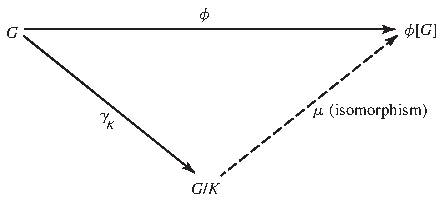
\includegraphics[width=0.602\linewidth,height=.8\textheight,keepaspectratio]{assets/p134_11.pdf}\end{center}
\begin{center}\small\textbf{12.15 Figure}\end{center}
\end{BookFloat}

\end{BookBody}

% Source PDF page 135; original printed page 118
\BookSource{135}{118}
\BookNarrativetrue

\begin{BookBody}

\BookLabel{12.16 Example} Classify the group \BookInline{(\mathbb{Z}_{4}\times \mathbb{Z}_{2})/(\{0\}\times \mathbb{Z}_{2})} according to the fundamental theorem of finitely generated abelian groups (Theorem 9.12).

\BookLabel{\textit{Solution}} The projection map \BookInline{\pi _{1}:\mathbb{Z}_{4}\times \mathbb{Z}_{2}\to \mathbb{Z}_{4}} given by \BookInline{\pi _{1}(x,\allowbreak y)= x} is a homomorphism of \BookInline{\mathbb{Z}_{4}\times \mathbb{Z}_{2}} onto \BookInline{\mathbb{Z}_{4}} with kernel \BookInline{\{0\}\times \mathbb{Z}_{2}.} By Theorem 12.14, we know that the given factor group is isomorphic to \BookInline{\mathbb{Z}_{4}.}\BookEnd{\blacktriangle}

\BookTextHeading{\textbf{Normal Subgroups and Inner Automorphisms}  }

\noindent We derive some alternative characterizations of normal subgroups, which often provide us with an easier way to check normality than finding both the left and the right coset decompositions.

Suppose that \BookInline{H} is a subgroup of \BookInline{G} such that \BookInline{ghg^{- 1}\in H} for all \BookInline{g\in G} and all \BookInline{h\in H.} Then \BookInline{gHg^{- 1}= \{ghg^{- 1}\mid h\in H\}\subseteq H} for all \BookInline{g\in G.} We claim that actually \BookInline{gHg^{- 1}= H.} We must show that \BookInline{H\subseteq gHg^{- 1}} for all \BookInline{g\in G.} Let \BookInline{h\in H.} Replacing \BookInline{g} by \BookInline{g^{- 1}} in the relation \BookInline{ghg^{- 1}\in H,\allowbreak } we obtain \BookInline{g^{- 1}h(g^{- 1})^{- 1}= g^{- 1}hg= h_{1}} where \BookInline{h_{1}\in H.} Consequently, \BookInline{h= gh_{1}g^{- 1}\in gHg^{- 1},\allowbreak } and we are done.

Suppose that \BookInline{gH= Hg} for all \BookInline{g\in G.} Then \BookInline{gh= h_{1}g,\allowbreak } so \BookInline{ghg^{- 1}\in H} for all \BookInline{g\in G} and all \BookInline{h\in H.} By the preceding paragraph, this means that \BookInline{gHg^{- 1}= H} for all \BookInline{g\in G.} Conversely, if \BookInline{gHg^{- 1}= H} for all \BookInline{g\in G,\allowbreak } then \BookInline{ghg^{- 1}= h_{1}} so \BookInline{gh= h_{1}g\in Hg,\allowbreak } and \BookInline{gH\subseteq Hg.} But also\BookInline{,\allowbreak g^{- 1}Hg= H} giving \BookInline{g^{- 1}hg= h_{2},\allowbreak } so that \BookInline{hg= gh_{2}} and \BookInline{Hg\subseteq } \BookInline{gH.}

The comments after Definition 12.3 show that the kernel of any homomorphism is a normal subgroup of the domain. Also, Theorem 12.12 says that any normal subgroup is the kernel of some homomorphism.

We summarize our work as a theorem.

\BookLabel{12.17 Theorem} The following are four equivalent conditions for a subgroup \BookInline{H} of a group \BookInline{G} to be a \textit{normal} subgroup of \BookInline{G.}

\BookExercise{1.}{\BookInline{ghg^{- 1}\in H} for all \BookInline{g\in G} and \BookInline{h\in H.}}

\BookExercise{2.}{\BookInline{gHg^{- 1}= H} for all \BookInline{g\in G.}}

\BookExercise{3.}{There is a group homomorphism \BookInline{\phi:G\to G^{\prime }} such that Ker\BookInline{(\phi )= H.}}

\BookExercise{4.}{\BookInline{gH= Hg} for all \BookInline{g\in G.}}

\noindent Condition (2) of Theorem 12.17 is often taken as the definition of a normal subgroup \BookInline{H} of a group \BookInline{G.}\BookEnd{\blacklozenge}

\BookLabel{12.18 Example} Every subgroup \BookInline{H} of an abelian group \BookInline{G} is normal. We need only note that \BookInline{gh= hg} for all \BookInline{h\in H} and all \BookInline{g\in G,\allowbreak } so, of course\BookInline{,\allowbreak ghg^{- 1}= h\in H} for all \BookInline{g\in G} and all \BookInline{h\in H.}\BookEnd{\blacktriangle}

If \BookInline{G} is a group and \BookInline{g\in G,\allowbreak } then the map \BookInline{i_{g}:G\to G} defined by \BookInline{i_{g}(x)= gxg^{- 1}} is a group homomorphism since \BookInline{i_{g}(xy)= gxyg^{- 1}= gxg^{- 1}gyg^{- 1}= i_{g}(x)i_{g}(x).} We see that \BookInline{gag^{- 1}= gbg^{- 1}} if and only if \BookInline{a= b,\allowbreak } so \BookInline{i_{g}} is one-to-one. Since \BookInline{g(g^{- 1}yg)g^{- 1}= y,\allowbreak } we see that \BookInline{i_{g}} is onto \BookInline{G,\allowbreak } so it is an isomorphism of \BookInline{G} with itself.

\BookLabel{12.19 Definition} An isomorphism \BookInline{\phi:G\to G} of a group \BookInline{G} with itself is an\textbf{ automorphism} of \BookInline{G.} The automorphism \BookInline{i_{g}:G\to G,\allowbreak } where \BookInline{i_{g}(x)= gxg^{- 1}} for all \BookInline{x\in G,\allowbreak } is the\textbf{ inner automor}\textbf{phism of} \BookInline{G} \textbf{by} \BookInline{g.} Performing \BookInline{i_{g}} on \BookInline{x} is called\textbf{ conjugation of} \BookInline{x} \textbf{by} \BookInline{g.}\BookEnd{\blacksquare}

The equivalence of conditions (1) and (2) in Theorem 12.17 shows that \BookInline{gH= Hg} for all \BookInline{g\in G} if and only if \BookInline{i_{g}[H]= H} for all \BookInline{g\in G,\allowbreak } that is, if and only if \BookInline{H} is\textbf{ invariant} under all inner automorphisms of \BookInline{G.} It is important to realize that \BookInline{i_{g}[H]= H} is an 
% Source PDF page 136; original printed page 119
\BookSource{136}{119}
equation in\textit{ sets;} we need not have \BookInline{i_{g}(h)= h} for all \BookInline{h\in H.} That is \BookInline{i_{g}} may perform a nontrivial\textit{ permutation} of the set \BookInline{H.} We see that the normal subgroups of a group \BookInline{G} are precisely those that are invariant under all inner automorphisms. A subgroup \BookInline{K} of \BookInline{G} is a\textbf{ conjugate subgroup} of \BookInline{H} if \BookInline{K= i_{g}[H]= gHg^{- 1}} for some \BookInline{g\in G.}

\end{BookBody}

\BookNarrativetrue

\begin{BookBody}

\end{BookBody}

\BookNarrativefalse

\begin{BookBody}

\BookExerciseTitle{12}

\BookTextHeading{\textbf{Computations}}

\noindent In Exercises 1 through 8, find the order of the given factor group.

\BookExercise{1.}{\BookInline{\mathbb{Z}_{6}/\langle 3\rangle }}

\BookExercise{2.}{\BookInline{(\mathbb{Z}_{4}\times \mathbb{Z}_{12})/(\langle 2\rangle \times \langle 2\rangle )}}

\BookExercise{3.}{\BookInline{(\mathbb{Z}_{4}\times \mathbb{Z}_{2})/\langle (2,\allowbreak 1)\rangle }}

\BookExercise{4.}{\BookInline{(\mathbb{Z}_{3}\times \mathbb{Z}_{5})/(\{0\}\times \mathbb{Z}_{5})}}

\BookExercise{5.}{\BookInline{(\mathbb{Z}_{3}\times \mathbb{Z}_{6})/\langle (1,\allowbreak 1)\rangle }}

\BookExercise{6.}{\BookInline{(\mathbb{Z}_{50}\times \mathbb{Z}_{75})/\langle (15,\allowbreak 15)\rangle }}

\BookExercise{7.}{\BookInline{(\mathbb{Z}_{26}\times \mathbb{Z}_{15})/\langle (1,\allowbreak 1)\rangle }}

\BookExercise{8.}{\BookInline{(\mathbb{Z}_{8}\times S_{3})/\langle (2,\allowbreak (1,\allowbreak 2,\allowbreak 3))\rangle } In Exercises 9 through 15, give the order of the element in the factor group.}

\BookExercise{9.}{\BookInline{5+ \langle 4\rangle } in \BookInline{\mathbb{Z}_{12}/\langle 4\rangle }}

\BookExercise{10.}{\BookInline{26+ \langle 12\rangle } in \BookInline{\mathbb{Z}_{60}/\langle 12\rangle }}

\BookExercise{11.}{\BookInline{(2,\allowbreak 1)+ \langle (1,\allowbreak 1)\rangle } in \BookInline{(\mathbb{Z}_{3}\times \mathbb{Z}_{6})/\langle (1,\allowbreak 1)\rangle }}

\BookExercise{12.}{\BookInline{(3,\allowbreak 1)+ \langle (1,\allowbreak 1)\rangle } in \BookInline{(\mathbb{Z}_{4}\times \mathbb{Z}_{4})/\langle (1,\allowbreak 1)\rangle }}

\BookExercise{13.}{\BookInline{(2,\allowbreak 3)+ \langle (0,\allowbreak 3)\rangle } in \BookInline{(\mathbb{Z}_{10}\times \mathbb{Z}_{4})/\langle (0,\allowbreak 3)\rangle }}

\BookExercise{14.}{\BookInline{(2,\allowbreak 5)+ \langle (1,\allowbreak 2)\rangle } in \BookInline{(\mathbb{Z}_{3}\times \mathbb{Z}_{6})/\langle (1,\allowbreak 2)\rangle }}

\BookExercise{15.}{\BookInline{(2,\allowbreak 0)+ \langle (4,\allowbreak 4)\rangle } in \BookInline{(\mathbb{Z}_{6}\times \mathbb{Z}_{8})/\langle (4,\allowbreak 4)\rangle }}

\BookExercise{16.}{Compute \BookInline{i_{\rho }[H]} for the subgroup \BookInline{H= \{\iota,\allowbreak \mu \}} of the dihedral group \BookInline{D_{3}.}}

\BookTextHeading{\textbf{Concepts}}

\noindent In Exercises 17 through 19, correct the definition of the italicized term without reference to the text, if correction is needed, so that it is in a form acceptable for publication.

\BookExercise{17.}{A\textit{ normal subgroup} \BookInline{H} of \BookInline{G} is one satisfying \BookInline{hG= Gh} for all \BookInline{h\in H.}}

\BookExercise{18.}{A\textit{ normal subgroup} \BookInline{H} of \BookInline{G} is one satisfying \BookInline{g^{- 1}hg\in H} for all \BookInline{h\in H} and all \BookInline{g\in G.}}

\BookExercise{19.}{An\textit{ automorphism} of a group \BookInline{G} is a homomorphism mapping \BookInline{G} into \BookInline{G.}}

\BookExercise{20.}{What is the importance of a\textit{ normal} subgroup of a group \BookInline{G}?}

\noindent Students often write nonsense when first proving theorems about factor groups. The next two exercises are designed to call attention to one basic type of error.

\BookExercise{21.}{A student is asked to show that if \BookInline{H} is a normal subgroup of an abelian group \BookInline{G,\allowbreak } then \BookInline{G/H} is abelian. The student’s proof starts as follows:}

\noindent We must show that \BookInline{G/H} is abelian. Let \BookInline{a} and \BookInline{b} be two elements of \BookInline{G/H.}

\BookExercise{a.}{Why does the instructor reading this proof expect to find nonsense from here on in the student’s paper?}

\BookExercise{b.}{What should the student have written?}

\BookExercise{c.}{Complete the proof.}

\BookExercise{22.}{A\textbf{ torsion group} is a group all of whose elements have finite order. A group is\textbf{ torsion free} if the identity is the only element of finite order. A student is asked to prove that if \BookInline{G} is a torsion group, then so is \BookInline{G/H} for every normal subgroup \BookInline{H} of \BookInline{G.} The student writes}

\noindent We must show that each element of \BookInline{G/H} is of finite order. Let \BookInline{x\in G/H.} Answer the same questions as in Exercise 21.

\BookExercise{23.}{Determine whether each of the following is true or false.}

\BookExercise{a.}{It makes sense to speak of the factor group \BookInline{G/N} if and only if \BookInline{N} is a normal subgroup of the group \BookInline{G.}}

\BookExercise{b.}{Every subgroup of an abelian group \BookInline{G} is a normal subgroup of \BookInline{G.}}

\BookExercise{c.}{The only automorphism of an abelian group is the identity map.}

\end{BookBody}

% Source PDF page 137; original printed page 120
\BookSource{137}{120}
\BookNarrativefalse

\begin{BookBody}

\BookExercise{d.}{Every factor group of a finite group is again of finite order.}

\BookExercise{e.}{Every factor group of a torsion group is a torsion group. (See Exercise 22.)}

\BookExercise{f.}{Every factor group of a torsion-free group is torsion free. (See Exercise 22.)}

\BookExercise{g.}{Every factor group of an abelian group is abelian.}

\BookExercise{h.}{Every factor group of a nonabelian group is nonabelian.}

\BookExercise{i.}{\textbf{i}\BookInline{.\mathbb{Z}/n\mathbb{Z}} is cyclic of order \BookInline{n.}}

\BookExercise{j.}{\textbf{j}\BookInline{.\mathbb{R}/n\mathbb{R}} is cyclic of order \BookInline{n,\allowbreak } where \BookInline{n\mathbb{R}= \{nr\mid r\in \mathbb{R}\}} and \BookInline{\mathbb{R}} is under addition.}

\BookTextHeading{\textbf{Theory}}

\BookExercise{24.}{Let \BookInline{G_{1}} and \BookInline{G_{2}} be groups and \BookInline{\pi _{1}:G_{1}\times G_{2}\to G_{1}} be the function defined by \BookInline{\pi _{1}(a,\allowbreak b)= a.} Prove that \BookInline{\pi _{1}} is a homomorphism, find Ker\BookInline{(\pi _{1}),\allowbreak } and prove \BookInline{(G_{1}\times G_{2})/}Ker\BookInline{(\pi _{1})} is isomorphic to \BookInline{G_{1}.}}

\BookExercise{25.}{Let \BookInline{G_{1}} and \BookInline{G_{2}} be groups and \BookInline{\phi:G_{1}\times G_{2}\to G_{1}\times G_{2}} be the function defined by \BookInline{\phi (a,\allowbreak b)= (a,\allowbreak e_{2})} where \BookInline{e_{2}} is the identity in \BookInline{G_{2}.} Prove that \BookInline{\phi } is a homomorphism, find Ker\BookInline{(\phi ),\allowbreak } and prove \BookInline{(G_{1}\times G_{2})/}Ker\BookInline{(\phi )} is isomorphic to \BookInline{G_{1}.}}

\BookExercise{26.}{Complete the proof of Theorem 12.7 by showing that if \BookInline{H} is a subgroup of a group \BookInline{G} and if left coset multiplication \BookInline{(aH)(bH)= (ab)H} is well defined, then \BookInline{Ha\subseteq aH.}}

\BookExercise{27.}{Prove that the torsion subgroup \BookInline{T} of an abelian group \BookInline{G} is a normal subgroup of \BookInline{G,\allowbreak } and that \BookInline{G/T} is torsion free. (See Exercise 22.)}

\BookExercise{28.}{A subgroup \BookInline{H} is\textbf{ conjugate to a subgroup} \BookInline{K} of a group \BookInline{G} if there exists an inner automorphism \BookInline{i_{g}} of \BookInline{G} such that \BookInline{i_{g}[H]= K.} Show that conjugacy is an equivalence relation on the collection of subgroups of \BookInline{G.}}

\BookExercise{29.}{Characterize the normal subgroups of a group \BookInline{G} in terms of the cells where they appear in the partition given by the conjugacy relation in the preceding exercise.}

\BookExercise{30.}{Find all subgroups of \BookInline{D_{3}} that are conjugate to \BookInline{H= \{\iota,\allowbreak \mu \}.(}See Exercise 28.)}

\BookExercise{31.}{\textbf{ (Evaluation Homomorphism)} Let \BookInline{F} be the set of all functions mapping the real numbers to the real numbers and let \BookInline{c\in \mathbb{R}.} The sum of two functions \BookInline{f+ g} is the function defined by \BookInline{(f+ g)(x)= f(x)+ g(x).} Function addition makes \BookInline{F} a group. Let \BookInline{\phi _{c}:F\to \mathbb{R}} be defined by \BookInline{\phi _{c}(f)= f(c).}}

\BookExercise{a.}{Show that \BookInline{\phi _{c}} is a group homomorphism.}

\BookExercise{b.}{Find Ker\BookInline{(\phi _{c}).}}

\BookExercise{c.}{Identify the coset of Ker\BookInline{(\phi _{c})} that contains the constant function \BookInline{f(x)= 1.}}

\BookExercise{d.}{Find a well-known group that is isomorphic with \BookInline{F/}Ker\BookInline{(\phi _{c}).} Use the Fundamental Homomorphism Theorem to prove your answer.}

\BookExercise{32.}{Let \BookInline{H} be a normal subgroup of a group \BookInline{G,\allowbreak } and let \BookInline{m= (G:H).} Show that \BookInline{a^{m}\in H} for every \BookInline{a\in G.}}

\BookExercise{33.}{Show that an intersection of normal subgroups of a group \BookInline{G} is again a normal subgroup of \BookInline{G.}}

\BookExercise{34.}{Given any subset \BookInline{S} of a group \BookInline{G,\allowbreak } show that it makes sense to speak of the smallest normal subgroup that contains \BookInline{S.[}\textit{Hint:} Use Exercise 33.]}

\BookExercise{35.}{Let \BookInline{G} be a group. An element of \BookInline{G} that can be expressed in the form \BookInline{aba^{- 1}b^{- 1}} for some \BookInline{a,\allowbreak b\in G} is a \textbf{commutator} in \BookInline{G.} The preceding exercise shows that there is a smallest normal subgroup \BookInline{C} of a group \BookInline{G} containing all commutators in \BookInline{G;} the subgroup \BookInline{C} is the\textbf{ commutator subgroup} of \BookInline{G.} Show that \BookInline{G/C} is an abelian group.}

\BookExercise{36.}{Show that if a finite group \BookInline{G} has exactly one subgroup \BookInline{H} of a given order, then \BookInline{H} is a normal subgroup of \BookInline{G.}}

\BookExercise{37.}{Show that if \BookInline{H} and \BookInline{N} are subgroups of a group \BookInline{G,\allowbreak } and \BookInline{N} is normal in \BookInline{G,\allowbreak } then \BookInline{H\cap N} is normal in \BookInline{H.} Show by an example that \BookInline{H\cap N} need not be normal in \BookInline{G.}}

\BookExercise{38.}{Let \BookInline{G} be a group containing at least one subgroup of a fixed finite order \BookInline{s.} Show that the intersection of all subgroups of \BookInline{G} of order \BookInline{s} is a normal subgroup of \BookInline{G.[}\textit{Hint:} Use the fact that if \BookInline{H} has order \BookInline{s,\allowbreak } then so does \BookInline{x^{- 1}Hx} for all \BookInline{x\in G.]}}

\end{BookBody}

% Continuation on source PDF page 138, preceding Section 13
\BookNarrativefalse

\begin{BookBody}

\BookExercise{39.}{\textbf{. a} Show that all automorphisms of a group \BookInline{G} form a group under function composition.}

\BookExercise{b.}{Show that the inner automorphisms of a group \BookInline{G} form a normal subgroup of the group of all automorphisms of \BookInline{G} under function composition. [\textit{Warning:} Be sure to show that the inner automorphisms do form a subgroup.]}

\BookExercise{40.}{Show that the set of all \BookInline{g\in G} such that \BookInline{i_{g}:G\to G} is the identity inner automorphism \BookInline{i_{e}} is a normal subgroup of a group \BookInline{G.}}

\BookExercise{41.}{Let \BookInline{G} and \BookInline{G^{\prime }} be groups, and let \BookInline{H} and \BookInline{H^{\prime }} be normal subgroups of \BookInline{G} and \BookInline{G^{\prime },\allowbreak } respectively. Let \BookInline{\phi } be a homomorphism of \BookInline{G} into \BookInline{G^{\prime }.} Show that \BookInline{\phi } induces a natural homomorphism \BookInline{\phi _{\ast }:(G/H)\to (G^{\prime }/H^{\prime })} if \BookInline{\phi [H]\subseteq H^{\prime }.} (This fact is used constantly in algebraic topology.)}

\BookExercise{42.}{Use the properties det\BookInline{(AB)= } det\BookInline{(A)\cdot } det\BookInline{(B)} and det\BookInline{(I_{n})= 1} for \BookInline{n\times n} matrices to show the \BookInline{n\times n} matrices with determinant \BookInline{\pm 1} form a normal subgroup of GL\BookInline{(n,\allowbreak \mathbb{R}).}}

\BookExercise{43.}{Let \BookInline{G} be a group, and let \BookInline{\mathcal{P}(G)} be the set of all\textit{ subsets} of \BookInline{G.} For any \BookInline{A,\allowbreak B\in \mathcal{P}(G),\allowbreak } let us define the product subset \BookInline{AB= \{ab\mid a\in A,\allowbreak b\in B\}.}}

\BookExercise{a.}{Show that this multiplication of subsets is associative and has an identity element, but that \BookInline{\mathcal{P}(G)} is not a group under this operation.}

\BookExercise{b.}{Show that if \BookInline{N} is a normal subgroup of \BookInline{G,\allowbreak } then the set of cosets of \BookInline{N} is closed under the above operation on \BookInline{\mathcal{P}(G),\allowbreak } and that this operation agrees with the multiplication given by the formula in Corollary 12.8.}

\BookExercise{c.}{Show (without using Corollary 12.8) that the cosets of \BookInline{N} in \BookInline{G} form a group under the above operation. Is its identity element the same as the identity element of \BookInline{\mathcal{P}(G)}?}

\end{BookBody}
\ifdefined\BookMaster\let\BookFinish\relax\else\def\BookFinish{\end{document}}\fi\BookFinish
